% --------------------------------------------------
% 
% This chapter is for HPC
% 
% --------------------------------------------------

\chapter{Computing resources: a  prerequisite \& a limitation in modern microbial ecology}
\label{cha:6}


\section{0s and 1s in marine molecular research}

HPC paper

\begin{figure}{}
   \centering
   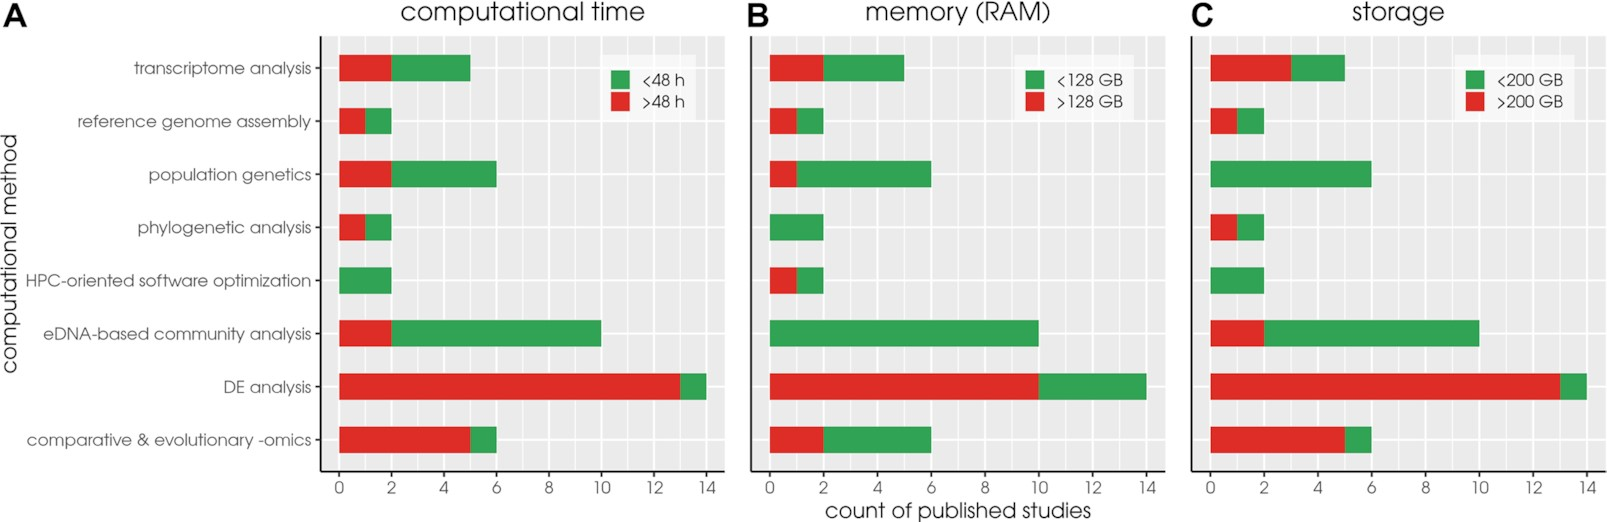
\includegraphics[width=140mm]{figures/zorbas_jobs_resources.jpeg}
   \caption{Red bars denote published research with high resource requirements of the various computational methods employed at the IMBBC HPC facility due to (a) long computational times (>48 h), (b) high memory requirements (>128 GB), or (c) high storage requirements (>200 GB). For instance, no eDNA-based community analyses performed at Zorba thus far have required a large amounts of memory.}
   \label{fig:zorba_jobs}
\end{figure}



Infrustuctures could be of use

